\documentclass[11pt]{article}
\usepackage[utf8]{inputenc} %Input encoding

\usepackage{amsmath} %Extra math symbols and operators
\usepackage{amssymb}
\usepackage{amsthm}
\usepackage{eufrak}

\usepackage{bm} %Bold symbols

\usepackage{graphicx} %Images

\usepackage{tikz-cd} %Diagrams

\usepackage{enumitem} %Enumerate Labels

\usepackage[margin=1.5in]{geometry} %Adjust Margins

\usepackage{siunitx} % easily format numbers with dimensions
\usepackage{cleveref}

%\usepackage{fancyhdr} %Name on every page
%\pagestyle{fancy}
%\lhead{Rune Buckinx}

\usepackage{mdframed}
\newmdtheoremenv{definition}{Definition}[section]
\newmdtheoremenv{question}{Question}[section]
\newmdtheoremenv{lemma}{Lemma}[section]
\newmdtheoremenv{proposition}{Proposition}[section]
\newtheorem{example}{Example}[section]
\newtheorem{remark}{Remark}[section]
\newmdtheoremenv{theorem}{Theorem}[section]
\newmdtheoremenv{exercise}{Exercise}

\usepackage{import}
\usepackage{xifthen}
\usepackage{pdfpages}
\usepackage{transparent}

\newcommand{\incfig}[1]{
    \def\svgwidth{\columnwidth}
    \import{./figures/}{#1.pdf_tex}
}

\usepackage[backend=biber]{biblatex}
\addbibresource{references.bib}
%\tikzset{component/.style={draw,thick,circle,fill=white,minimum size =0.75cm,inner sep=0pt}}

\title{Modeling of MHD waves in the solar corona}
\author{Micha\"el Maex \and Rune Buckinx}
\date{March 2020}

\begin{document}

\maketitle

\begin{abstract}
    This paper presents a summary of research for a bachelor's thesis on the modelling of magnetohydrodynamic waves in the solar corona using numerical simulations via the open source code PLUTO. 
\end{abstract}
\tableofcontents
\newpage
\section{Introduction} \label{sec:introduction}
The Sun's corona, or solar corona, is the outer layer of the Sun's atmosphere, which consists of fully ionized material due to it having very high temperatures compared to the surface of the sun. The plasma in the solar corona can be described using magnetohydrodynamic (MHD) equations, which combine the Navier-Stokes equations from fluid dynamics with the Maxwell equations from electromagnetism. This approach to model the plasma treats it as a single fluid, as opposed to the two-fluid model, which describes the ions and electrons seperately. \\

The differential/governing equations that make up the MHD model, are difficult to solve analytically. It is therefore favorable to use numerical computer modeling to study the equations, which is the main focus of this bachelor's project. The simulations will be performed in the open source code PLUTO, which is designed to solve systems of partial differential equations in astrophysical fluid dynamics \cite{mignone2011pluto}. 
\section{Magnetohydrodynamics and the solar corona} \label{sec:magnetohydrodynamics_and_the_solar_corona}
The classic Navier-Stokes equations do not suffice to describe the movement in the solar corona due to the influence of strong magnetic fields on the ionized particles. This magnetic field stems from convection in the photosphere, which is a physical process that helps transport the nuclear energy created in the core of the sun \cite{brun2017magnetism}.\\

The use of the magnetohydrodynamic model to describe the plasma depends on three main assumptions, namely, high collisionality, large scales and the assumption of ideal fluids. The last assumption implies that the dissipation of large scale variables is neglected \cite{goedbloed2004principles}. This model also does not take relativity into account, as opposed to the relativistic magnetohydrodynamic model, which will not be discussed further \footnote{More information about the relativistic MHD model can be found in \cite{karas2005introduction}}.

Magnetohydrodynamics can be described by a system of partial differential equations. 
Just like ordinary fluid dynamics, these are derived from conservation laws. 
In this report we will only consider the non-relativistic approximation. 
The system of PDE's/conservations laws is the following:
\begin{alignat}{3}
    &\frac{\partial \rho}{\partial t} &&+ \nabla \cdot (\rho \mathbf v) &&= 0 \tag{mass}\label{masscont}\\
    &\frac{\partial \mathbf m}{\partial t} &&+  \nabla \cdot \bigg[\mathbf{mv - BB+ I}\bigg(p + \frac{\mathbf B^2}{2}\bigg)\bigg]^T &&= -\rho \nabla \Phi \tag{moment}\label{cauchymoment}\\
    &\frac{\partial \mathbf B}{\partial t} &&+ \nabla \times (cE) &&= 0 \tag{charge}\label{Faraday}\\
    &\frac{\partial(E_t + \rho \Phi)}{\partial t} &&+ \nabla \cdot \bigg[\bigg(\frac{\rho \mathbf v^2}{2} + \rho e + p + \rho \Phi\bigg)v + c \mathbf E \times \mathbf B\bigg] &&= 0 \tag{energy}\label{energy}.
\end{alignat}
Here $\rho$ is the plasma density, $\mathbf B$ is the magnetic field,  $\mathbf v$ the velocity, $\mathbf m= \rho \mathbf v$ the momentum density,$\Phi$ the potential, $p$ is the thermal pressure, $E_t$ is the total energy, which is given by \[
E_t, = \rho e \frac{m^2}{2\rho} + \frac{B^2}{2}
.\]  
The constants  $e, c$ are the elementary charge and the speed of light respectively.

If the environment is one where the thermal pressure and density are small deviations of some constant background pressure and density, $p_0, \rho_0$. Then the speed of sound is given by \[
c_s^2 = \gamma \frac{p_0}{\rho_0}
,\]
where $\gamma = \frac{f + 2}{f}, $ with $f$ the degrees of freedom of a particle. In a plasma $f$ is almost always $3$. 



\section{Pluto Code} \label{sec:pluto_code}

\subsection{Units in Pluto} \label{sec:units_in_pluto}

Internally Pluto uses dimensionless code units. All units are derived from the constants \texttt{UNIT\_DENSITY} ($\rho_0$), \texttt{UNIT\_LENGTH} ($L_0$), \texttt{UNIT\_VELOCITY} ($v_0$), all of which are denoted in cgs units. All other units are derived from these units.  
Note that the unit for magnetic field is defined as $B_0 = v_0\sqrt{4\pi \rho_0} $.

\Cref{tab:default_units} show some import dimensions in (M)HD and what one code unit represents when \texttt{UNIT\_DENSITY}, \texttt{UNIT\_LENGTH} and  \texttt{UNIT\_VELOCITY} have their default values.
\begin{table}[htpb]
	\centering
	\caption{Important dimensions and their code units in PLUTO}
	\label{tab:default_units}
	\begin{tabular}{c|c}
		one code unit of & corresponds to\\
		\hline 
		density & $m_p$ \si{\per \centi\metre\cubed} = \SI{1.67262171e-24}{\gram \per \centi\metre\cubed}\\
		lenth &\SI{1}{AU} \\
		velocity & \SI{1}{\kilo\metre \per \second}\\
		time & \SI{149597892}{\second} \\
		magnetic field strength & \SI{4.584624773e-07}{Gs} \\
		pressure & \SI{1.67262171e-14}{Ba} = \SI{1.6726217e-15}{Pa}
	\end{tabular}
\end{table}

\textcolor{red}{Hier iets schrijven over de units mss?}. 


\subsection{Initial example} \label{sec:initial_example}
The first problem that will be analysed is a simple hydrodynamic blastwave generated by a high-pressure region.  This problem is meant to be an initial example of how to set up a non-predefined simulation and is fully described in PLUTO's User Guide \cite{plutouserguide}. The blastwave is simulated in two dimensions and uses three user-defined parameters, namely, the ambient pressure, the pressure in the high-pressure region, and $\gamma$ which in this \textcolor{red}{paper/project?} will always be $5/3$. The domain goes from -10 to 10, in both the $x$ and the $y$ direction, with \textcolor{red}{200} points in both dimensions. The following initial condition is used, a high-pressure region inside a circle of radius 0.3 is surrounded by an ambient pressure region. The simulation is run for X units of time, and every Y units, a double-precision file is saved.
\section{Waves in magnetohydrodynamic fluids} \label{sec:waves_in_magnetorhydrodynamic_fluids}
In order to study the effects of a constant magnetic background field, the same initial conditions as in \cref{sec:initial_example} were used but this time a magnetic field in the $x$ direction was added.
The parameter $\mu = \frac{B^2}{2\pi p}$ gives the ratio of magnetic pressure over mechanical pressure. If $\mu = 0$ the magnetic field is $0$. If $\mu \gg 1$ the magnetic pressure dominates. \Cref{fig:blastwave_shape_mu} shows how the value of $\mu$ influences the shape of the blastwave.
\begin{figure}[h]
	\centering
	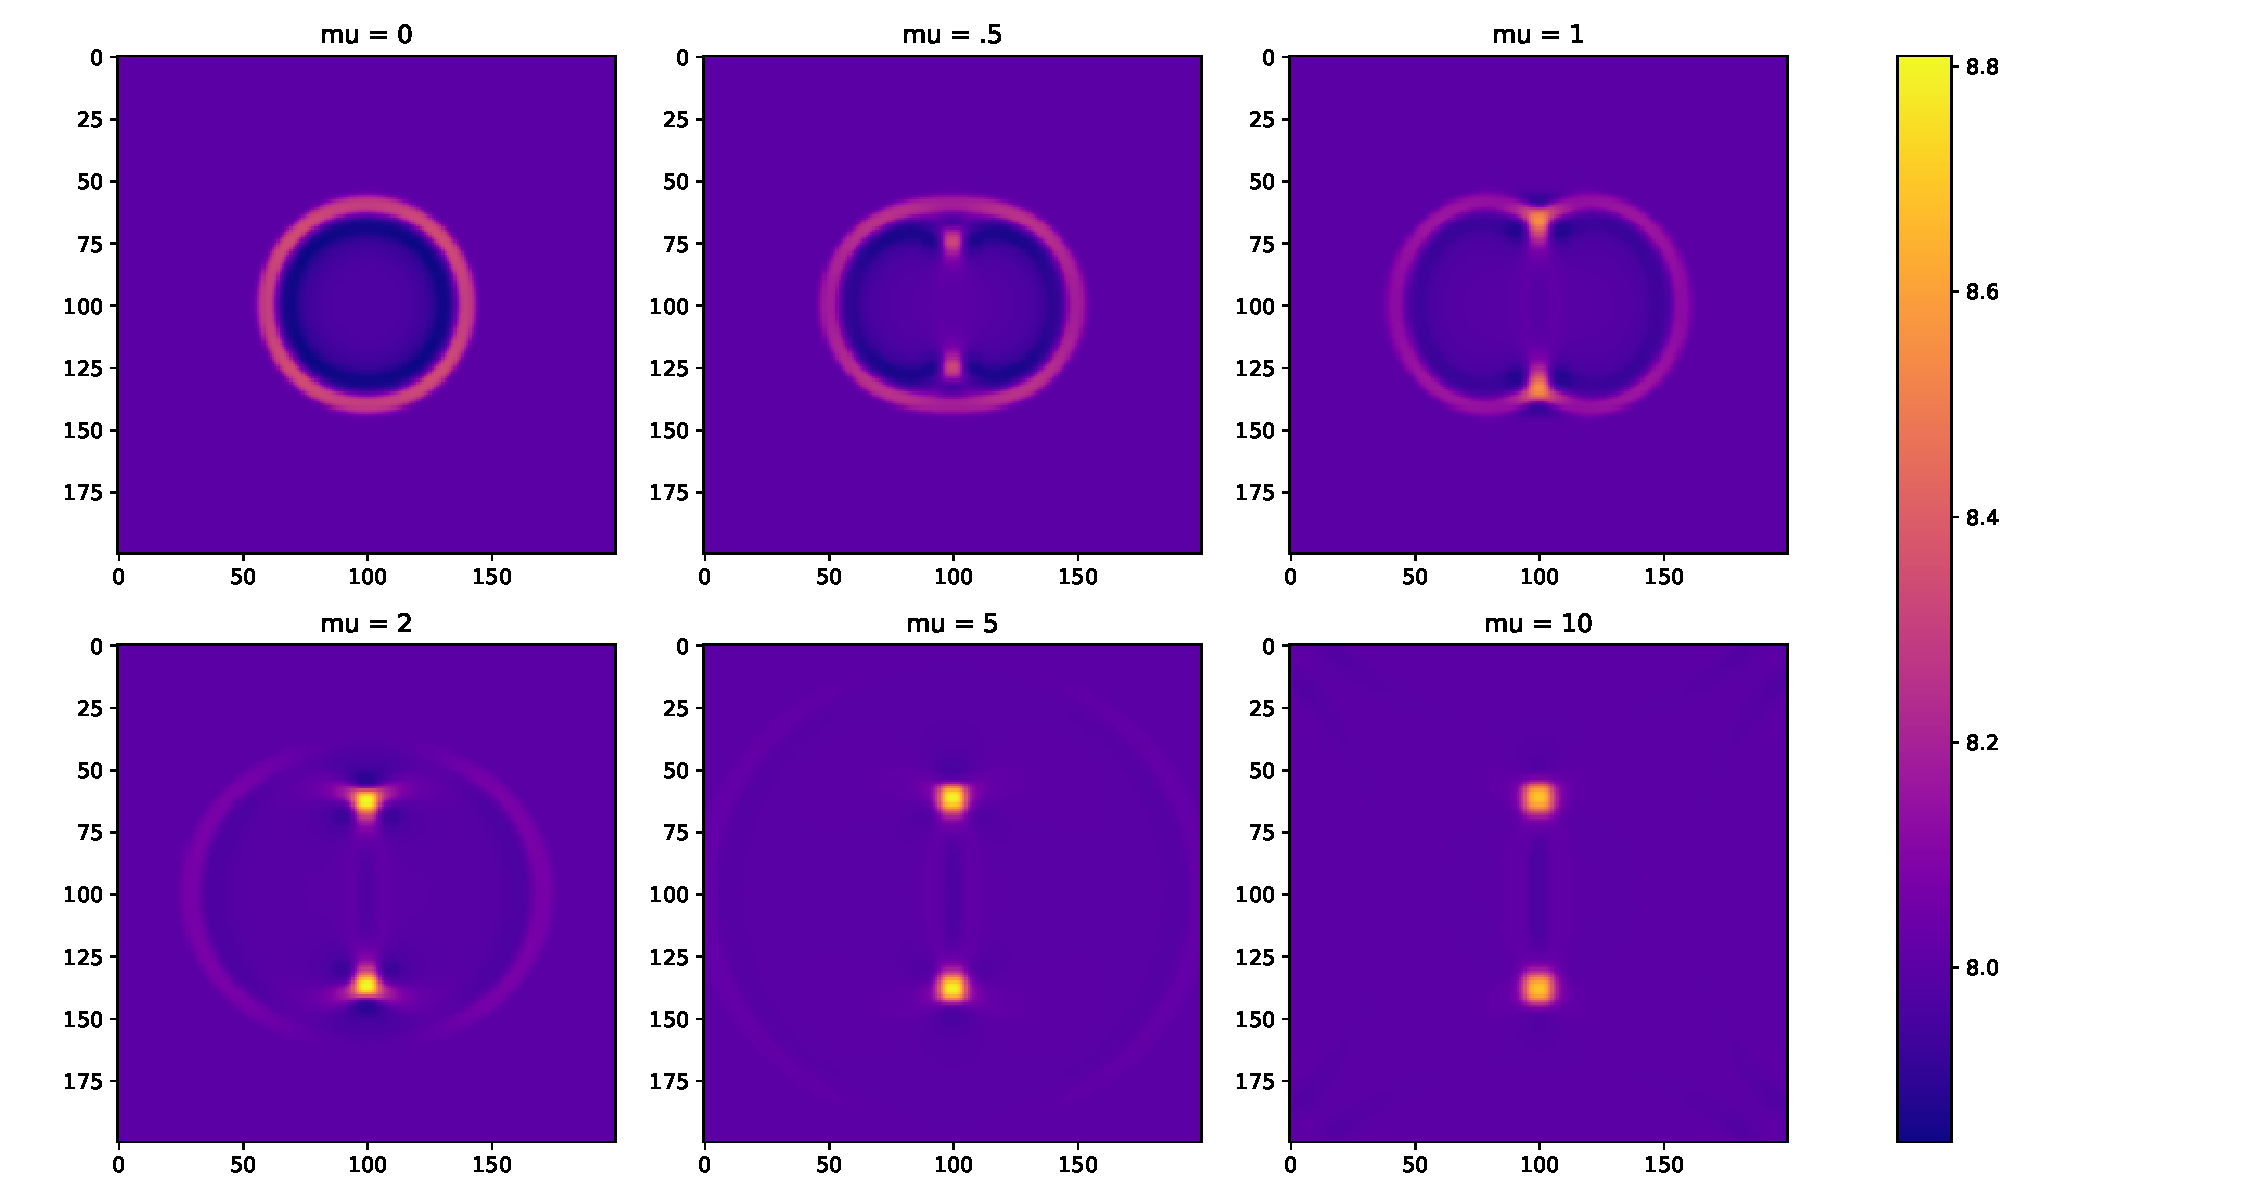
\includegraphics[width = \linewidth]{figures/influence_mu.pdf}
	\caption{}
\label{fig:blastwave_shape_mu}
\end{figure}
\section{Interaction of MHD waves with large scale structures}
Task 3
\section{Optional: MHD waves in slab geometry}
Task 4
\printbibliography
\end{document}
